%% To get pdf-file:    (acroread below allows you to look at pdf-file)
%====================
% (A) if your figures are ps-files or eps-files  (and not pdf,png,jpeg,etc.):
%---------------------------------------------------------------------
% latex trafficflowtalk.tex ;trafficflowtalk.tex ; dvips trafficflowtalk.dvi -o ; ps2pdf trafficflowtalk.ps ; acroread trafficflowtalk.pdf
% 
% (B) if your figures are pdf,png,jpeg etc (and not ps-files or eps-files)
%---------------------------------------------------------------------
% pdflatex beamer_example.tex 
%
\documentclass[t]{beamer}
% Ben's option:
\usecolortheme{whale}       
% Sophie's option:
%\usepackage{beamerthemeBerkeley}
%
\usefonttheme[onlymath]{serif}   
\usepackage{graphicx}
\usepackage{listings}
\usepackage{caption}
\usepackage{braket}

\usepackage{subfig}
\usepackage{commath}

\setbeamertemplate{navigation symbols}{}  % turns off annoying nav. symbols

\title{Real Time Signal Processing with Symmetric and Asymmetric Support Intervals}
\author{Kevin Joyce and Lia Harrington \\
       University of Montana}
\date{May 14, 2015}
 
% for a recurring outline
% (this defines, what happens whenever you use \section{...}, namely
%     slide is created with title "Universality ..." and table of contents
%     which includes all section titles and highlights current section)
\AtBeginSection[]  
{
\begin{frame}
\frametitle{Outline} 
\tableofcontents[currentsection] 
\end{frame}  
}

\begin{document}
\definecolor{mygreen}{RGB}{28,172,0} % color values Red, Green, Blue
\definecolor{mylilas}{RGB}{170,55,241}
\lstset{language=Matlab,%
    basicstyle=\ttfamily\small,
    frame=single,%
    breaklines=true,%
    morekeywords={matlab2tikz},
    keywordstyle=\color{blue},%
    morekeywords=[2]{1}, keywordstyle=[2]{\color{black}},
    identifierstyle=\color{black},%
    stringstyle=\color{mylilas},
    commentstyle=\color{mygreen},%
    showstringspaces=false,%without this there will be a symbol in the places where there is a space
    emph=[1]{for,end,break},emphstyle=[1]\color{red}, %some words to emphasise
}

%%%%%%%%%%%%%%%%%%%%%%%%%%%%%%%%%%%%%%%%%%%%%%%%%%%%%%%%%%%%%%
\begin{frame}
\titlepage
\end{frame}
%%%%%%%%%%%%%%%%%%%%%%%%%%%%%%%%%%%%%%%%%%%%%%%%%%%%%%%%%%%%%
\section{Introduction and Motivation}
%%%%%%%%%%%%%%%%%%%%%%%%%%%%%%%%%%%%%%%%%%%%%%%%%%%%%%%%%%%%%
\begin{frame}
\frametitle{Importance of Real Time Signal Processing}
\vspace{.3cm}
\structure{What is real time signal processing?}
\vspace{.3cm}
\begin{itemize}
\item Applications
\begin{itemize}
\item Speech recognition
\item Audio signal processing
\item Video compression
\item Weather forecasting
\item Economic forecasting
\item Medical imagining (e.g., CAT, MRI)
\item And more...
\end{itemize}
\end{itemize}
\end{frame}
%%%%%%%%%%%%%%%%%%%%%%%%%%%%%%%%%%%%%%%%%%%%%%%%%%%%%%%%%%%%
\section{Problem Outline}
%%%%%%%%%%%%%%%%%%%%%%%%%%%%%%%%%%%%%%%%%%%%%%%%%%%%%%%%%%%%
\begin{frame}
\frametitle{What is the problem?}
\structure{Goal:} We wish to reconstruct some generated signal $\hat{x}$ that has been distorted by some error and convolution processes. \newline \vspace{.5cm}

\structure{Solution:} Find the ``convolution inverse'' of $a$. We call this the reconstruction operator $R$.
%%%%%%%%%%%%%%%%%%%%%%%%%%%%%%%%%%%%%%%%%%%%%%%%%%%%%%%%%%%%
\end{frame}
\begin{frame}
  \frametitle{Reconstruction Operator $R$}  
  \begin{itemize}
    \item Following Lecture 13, we seek a linear reconstruction operator $R$ that we assume is given by convolution with some $r$ supported on a specified interval $\Delta$, so that $\widehat x = r*x$.
    \item It was shown that such an operator satisfies
    $$
      H(r) = E( \widehat x - x )^2 = \Big\langle P (r - P^{-1}q), r- P^{-1}q \Big\rangle_{\Delta} + f_0 - \Big\langle q, P^{-1}q\Big\rangle_{\Delta}
    $$
    where $P$ is the operator associated with convolution by $p = a*\phi*a^* + \sigma^2\delta$ and $q = a*\phi$.
    \item So, for a given $\Delta$ support for $r$, the reconstruction kernel is uniquely determined by \alert{$r = P^{-1}q|_\Delta$}, and 
    $$
    \mathrm{Var}\, \widehat x = H_{min} = \alert{f_0 - \Big\langle q, P^{-1}q\Big\rangle_{\Delta}}.
    $$
  \end{itemize}
\end{frame}
%%%%%%%%%%%%%%%%%%%%%%%%%%%%%%%%%%%%%%%%%%%%%%%%%%%%%%%%%%%%
\section{Problem Approach and Steps} 
%%%%%%%%%%%%%%%%%%%%%%%%%%%%%%%%%%%%%%%%%%%%%%%%%%%%%%%%%%%%
\begin{frame}
\frametitle{Problem Approach Overview}
\begin{enumerate}
\item Specify problem settings
\begin{itemize}
\item $y = a*x+\nu, \hspace{.2cm} \nu ~(0,\sigma^2\delta). $
\item $ \hat{x} = r*y$ 
\begin{itemize}
\item $ r = P^{-1}q$ 
\end{itemize}
\item Choose some $\Delta = [-d,d]$  $\rightarrow $ compute $ r = P^{-1}q|_\Delta$ 
\item Choose some $\Delta = [T,\tau]$  $\rightarrow $ compute $ r = P^{-1}q|_\Delta$ 
\end{itemize}
\item Compute ``optimal'' $\Delta$ for $r$ by
\begin{itemize}
\item $H(\Delta) = E(\hat{x}_{i} - x_{i})^2 = f_{0} - \braket{q,P^{-1}q}_\Delta$
\item Plot $H(\Delta)$ vs either $d$ in the symmetric case,  or $(T,\tau)$ in the asymmetric case.
\end{itemize}
\item Choose ``optimal'' $\Delta \rightarrow$ compute $\widehat x = r * y$.
\item Illustrate the result of estimation with uncertainty given by
\begin{itemize}
\item $\sqrt{E(\hat{x}_{i} - x_{i}})^2 = \sqrt{H}$
\end{itemize}
\end{enumerate}
\end{frame}
%%%%%%%%%%%%%%%%%%%%%%%%%%%%%%%%%%%%%%%%%%%%%%%%%%%%%%%%%%%%
\begin{frame}
\frametitle{Problem Strategy: Step 1}
\structure{Specify the main ingredients of simulated measurement system:}
\begin{itemize}
\item Specify point spread function (influence function ) a, 
\begin{itemize}
\item Symmetric
\item Asymmetric
\end{itemize}
\item Covariance function $\phi$ for the signal $x$: 
\begin{equation}
\phi = \mathrm{Cov}\,(x) = b*b^{*}
\end{equation}
\item Variance $\sigma^2$ of the independent components of the additive random noise $\nu$
\begin{equation}
y = a*x+\nu, \hspace{.2cm} \nu ~(0,\sigma^2\delta). 
\end{equation}
\item Choose support interval $\Delta = [-d,d] $ or $\Delta = [-T,\tau]$
\end{itemize}
\end{frame}
%%%%%%%%%%%%%%%%%%%%%%%%%%%%%%%%%%%%%%%%%%%%%%%%%%%%%%%%%%%%
\begin{frame}
\frametitle{Signal and Covariance Setup}

\begin{columns}[t]
\column{.9\textwidth}
\centering
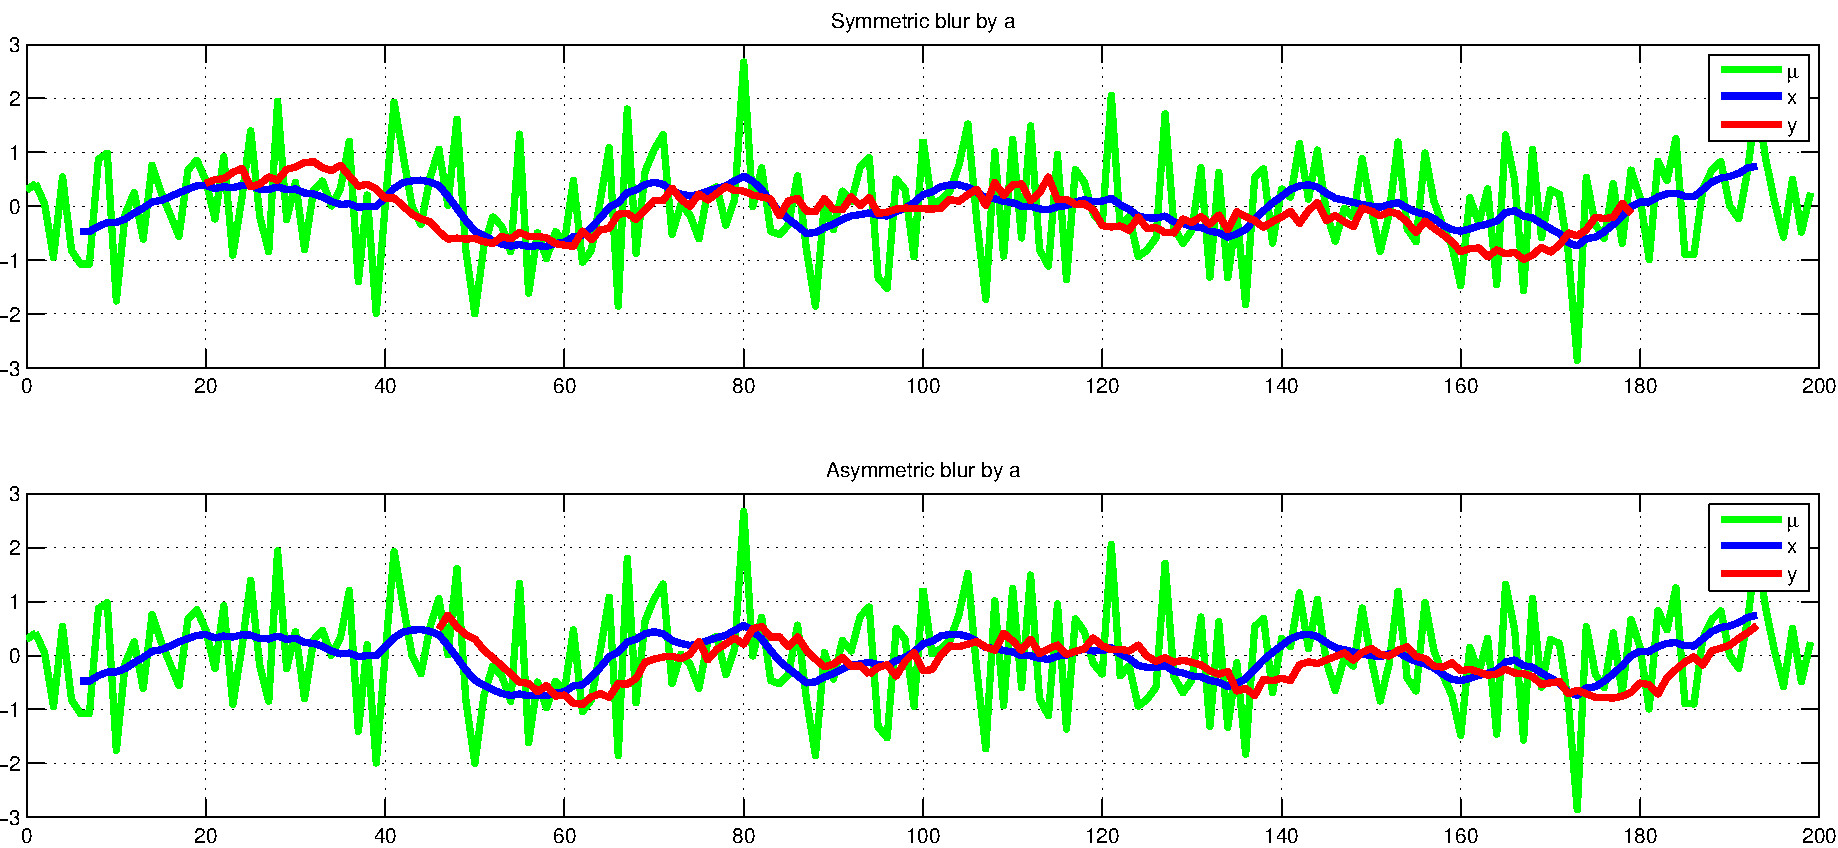
\includegraphics[scale=.3]{signal_setup.pdf}\\
%\vspace{.2cm}
%\column{.5\textwidth}
\includegraphics[scale=.3]{covariance_psf_setup.pdf}
\end{columns}

\end{frame}
%%%%%%%%%%%%%%%%%%%%%%%%%%%%%%%%%%%%%%%%%%%%%%%%%%%%%%%%%%%%
\begin{frame}
\frametitle{Problem Simulation}
\structure{Specify the main ingredients of simulated measurement system:}
\begin{itemize}
\item Finitely supported point spread function (influence function), 
  \begin{itemize}
    \item Symmetric case: \alert{$a_i = \frac 1{10}$} for $|i| < 15$.  
    \item Asymmetric case: \alert{$a_i = \frac 2{10} e^{-i/40}$} for $0\le i\le 40$.
  \end{itemize}
\item The covariance function $\phi$ for the signal $x$ is given by 
$$
\phi = \mathrm{Cov}\,(x) = b*b^{*}
$$
  where \alert{$b_i = \frac {21}{100}(1-|i|)$} for $|i| \le 7$. 
\item Measurement noise is modeled with a zero mean Gaussian $\nu$ with a specified \alert{$\sigma^2 = \frac 1{100}$}.
\item Finally, the data is given by
$$
  y = a * x + \nu
$$
\end{itemize}
\end{frame}
%%%%%%%%%%%%%%%%%%%%%%%%%%%%%%%%%%%%%%%%%%%%%%%%%%%%%%%%%%%%
\section{Code Comments}
\begin{frame}[fragile]
\frametitle{ Finitely Supported Function Data Type }
\begin{itemize}
  \item The fundamental data type in \texttt{Matlab} is the ``matvec'' whose operations are not ``natural'' for finitely supported discrete functions. 
  \item \texttt{Matlab} supports object oriented programming which allows for the creation of a custom data type for which we can implement convolution as the natural multiplication.
\end{itemize}
%\lstinputlisting[language=Matlab,firstline=1,lastline=8]{../FinSupFun.m} 
\begin{lstlisting}[language=Matlab]
classdef FinSupFun % Finite Support Function
    properties (SetAccess = private)
...
    end
    
    methods
...
    end
end
\end{lstlisting}
\end{frame}
%%%%%%%%%%%%%%%%%%%%%%%%%%%%%%%%%%%%%%%%%%%%%%%%%%%%%%%%%%%%
\begin{frame}[fragile]
\frametitle{ Finitely Supported Function Data Type }
\begin{itemize}
  \item From the demo codes provided, convolution and addition were ``overrided'' to allow statements like
\end{itemize}
%\lstinputlisting[language=Matlab,firstline=1,lastline=8]{../FinSupFun.m} 
\begin{lstlisting}[language=Matlab,basicstyle=\footnotesize]
mu = FinSupFun(randn(1,N),0); % Construct finitely supported white noise
x = b .* mu; % Inner convolution
y0 = a .* x; 
y = y0 + FinSupFun(s*randn(size(y0.f)),y0.l); 
phi = b*b'; % Outer convolution
p = a*phi*a' + FinSupFun(s^2); 
q = phi*a'; 
\end{lstlisting}
\begin{itemize}
  \item Note that the $*$ and $.*$ operations now represent convolution between \texttt{FinSupFun} objects.
  \item This makes code easier to read and debug.
\end{itemize}
\end{frame}
%%%%%%%%%%%%%%%%%%%%%%%%%%%%%%%%%%%%%%%%%%%%%%%%%%%%%%%%%%%%
\begin{frame}[fragile]
\frametitle{ Finitely Supported Function Data Type }
\begin{itemize}
  \item We added the following methods
\end{itemize}
%\lstinputlisting[language=Matlab,firstline=1,lastline=8]{../FinSupFun.m} 
\begin{lstlisting}[language=Matlab,basicstyle=\tiny]
function c = restricted_to(a,l,r) % Restrict support to [l,r], if [l,r] is bigger than [a.l,a.r], then pad with zeroes.
    L = max(l,a.l);	% Left endpoint of restricted interval 
    R = min(r,a.r);	% Right endpoint of restricted interval 
    ...
end

function c = mldivide(a,b) % \ De-convolution by constructing toeplitz matrix. a must be symmetric 
  n = length(b.f);
  toeplitz_row = [a.f((a.r+1):end), zeros(1, n-(a.r))];% This needs to be from the center of p and padded with zeros
  ...
end
\end{lstlisting}
\begin{itemize}
\item so computing $P^{-1}q$ on a restriced interval are easily implemented as follows
\end{itemize}
\begin{lstlisting}[language=Matlab,basicstyle=\tiny]
q_delta1 = q.restricted_to(-d,d); % Restrict (or zero pad) to [-d,d].
q_delta2 = q.restricted_to(-T,tau); % Restrict (or zero pad) to [-T,tau].
r1 = p \ q_delta1; 
r2 = p \ q_delta2; 
\end{lstlisting}
\end{frame}
%%%%%%%%%%%%%%%%%%%%%%%%%%%%%%%%%%%%%%%%%%%%%%%%%%%%%%%%%%%%
\section{Results and Conclusions}
%%%%%%%%%%%%%%%%%%%%%%%%%%%%%%%%%%%%%%%%%%%%%%%%%%%%%%%%%%%%
\begin{frame}
\end{frame}
\frametitle{ Results }
\begin{frame}
%%%%%%%%%%%%%%%%%%%%%%%%%%%%%%%%%%%%%%%%%%%%%%%%%%%%%%%%%%%%
\frametitle{References}

[1] Golubtsov, P. (2015). Theoretical Big Data Analytics course notes.

\end{frame}

\end{document}




\end{document}
